% Условная компиляция для самостоятельной работы
\ifdefined\mainfile
    % Если это часть основного файла, не добавляем начало и конец документа
\else
    \documentclass[12pt, a4paper]{report}
    \usepackage{/Users/vladbelousov/Desktop/Semestr_4-FP-NSU/Настройка/library}
    \usepackage[utf8]{inputenc} % Подключение поддержки UTF-8
    \begin{document}
\fi

%%-------------------------------%%

\[ \begin{aligned}
\begin{cases}
    \displaystyle I[y] = \int_{x_0}^{x_1} F(x,y(x),y'(x))dx \\
    y(x_0)=y_0, \text{ } y(x_1)=y_1
\end{cases}
\quad (1)
\end{aligned} \] 

Найти функцию \( y(x) \)   такую, чтобы функционал \( I[y] \) принимал наибольшее или наименьшее значение. 

Необходимо найти условие локального экстремума: 

Если \( \tilde{y }       \)  экстремаль \( \Rightarrow \tilde{y }  \frac{\partial F }{\partial y} - \frac{d}{dx }  \frac{\partial F}{\partial y '} = 0 \quad (2)   \)

\begin{proof}[Докозательство формулы (2)]
    \[ I[\tilde{y}] \le I[y] , y = \tilde{y} + \varepsilon \eta , \varepsilon \in  (- \varepsilon_1, \varepsilon_1), \eta(x) \in C^2([x_0,x_1])  - \text{финитная }    \] 
    
    \begin{center}
        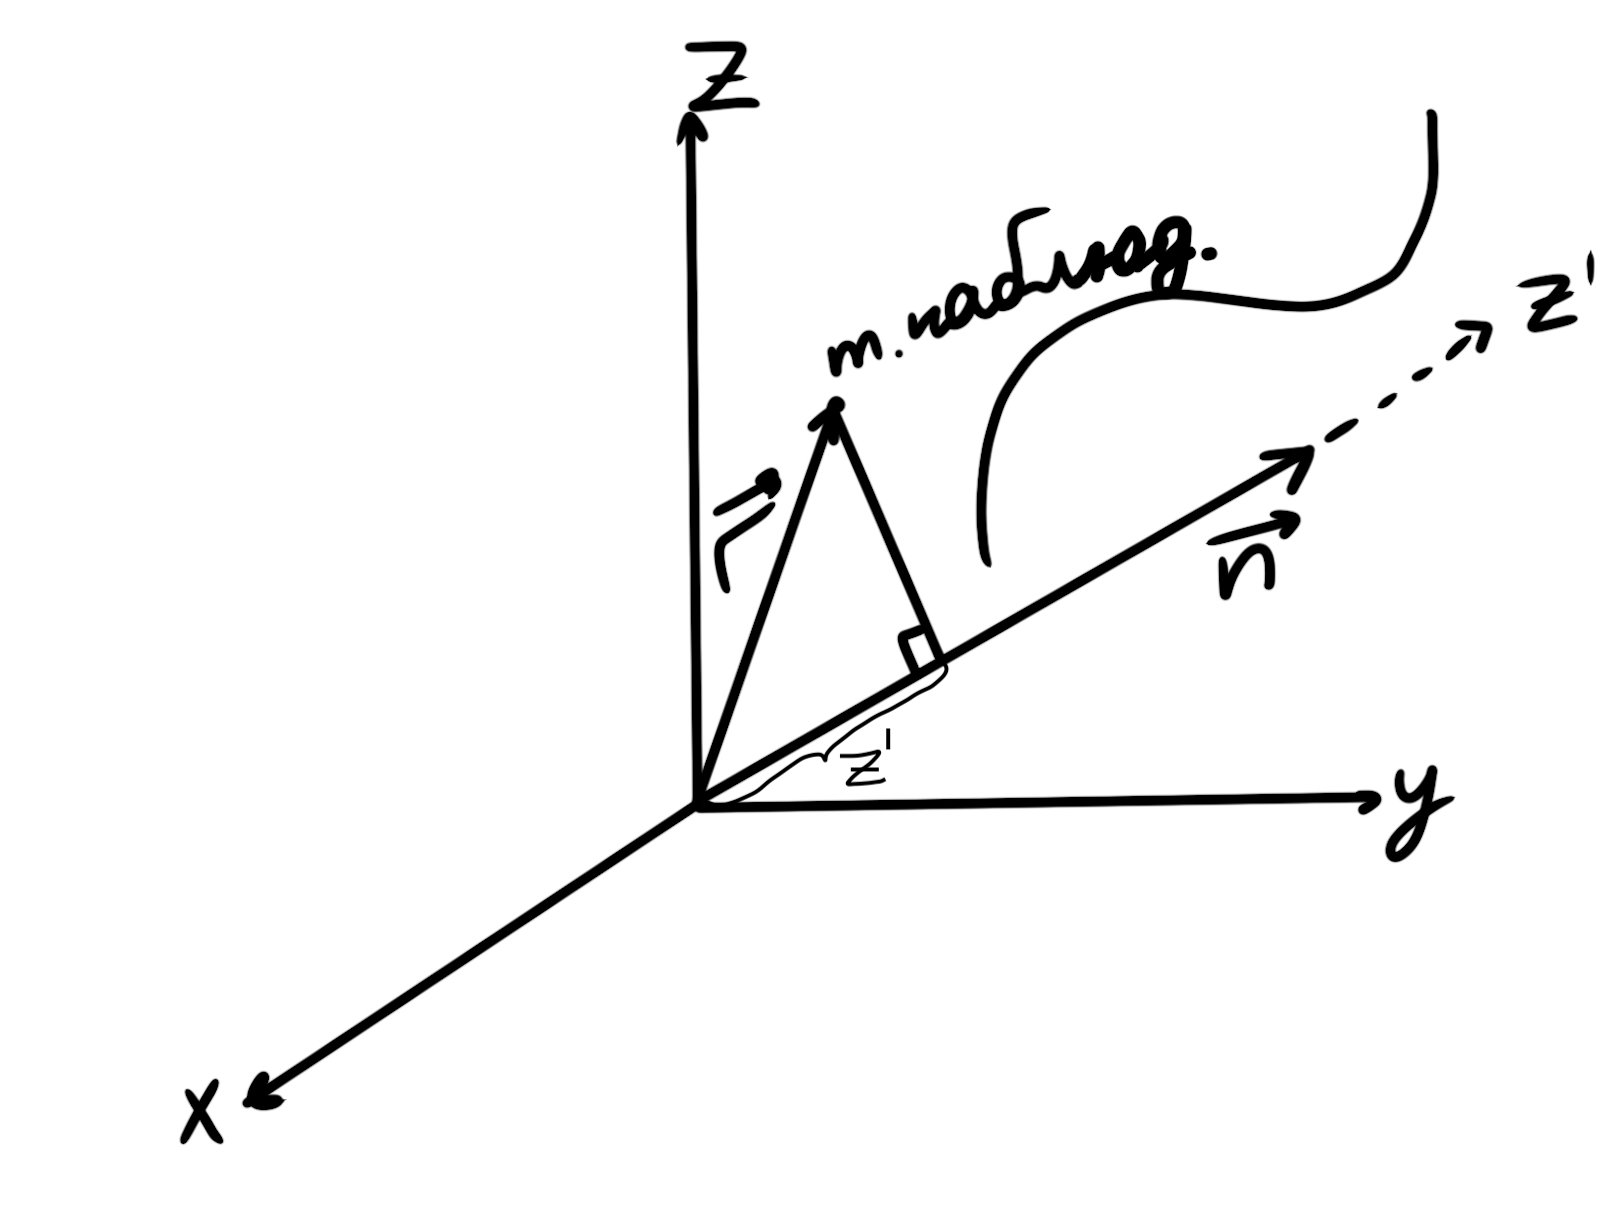
\includegraphics[width=0.3\textwidth]{/Users/vladbelousov/Desktop/Semestr_4-FP-NSU/ДфУ/Лекции_по_дням/image/7.png}
    \end{center}

    \[ \underbrace{I[y]}_{= g(0)} \le \underbrace{I[\tilde{y}+ \varepsilon \eta ]}_{=g(\varepsilon)} \Rightarrow g(0) \le g(\varepsilon) \Rightarrow g'( 0) = 0\] 

    \[ 0= \frac{d}{d \varepsilon} g(\varepsilon) |_{\varepsilon= 0 }= \int_{x_0}^{x_1} \left( \frac{\partial F }{\partial y } ( x , \tilde{y}(x) , \tilde{y }' (x) ) - \frac{d}{dx }  \frac{\partial F }{\partial y' } ( x , \tilde{y}(x) , \tilde{y }' (x) )  \right) \eta (x) dx , \forall \eta (x)  - \text{финитная}    \] 

    \begin{lemma}[Лагранжа]     
        Пусть \( f(x) \) - непрерывна и \( \displaystyle \int_{x_0}^{x_1} f(x) \eta (x) dx =0. \forall \eta (x) \) - финитная на \( [x_0,x_1] \). Тогда \( f(x) = 0 , \forall x \in  [x_0,x_1] \) 
    \end{lemma}

    \begin{proof}
        От противного:
        \begin{center}
            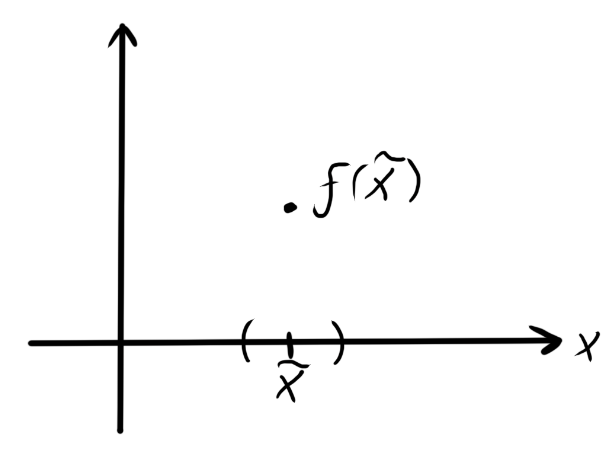
\includegraphics[width=0.3\textwidth]{/Users/vladbelousov/Desktop/Semestr_4-FP-NSU/ДфУ/Лекции_по_дням/image/8.png}
        \end{center}
        Пусть для определенности \( f(\tilde{x } )> 0        \) . Тогда так как \( f(\tilde{x}) \) - непрерывна, то \( f(x)>0    \) при \( x \in (\tilde{x}- \delta_0, \tilde{x}+\delta_0) \) 

        Возьмем функцию \( \eta(x) = \begin{aligned}
            \begin{cases}
                (\delta_0 ^2 - (x- \tilde{x})^2) ^ 4 , |x- \tilde{x}|< \delta   \\
                0 , |x- \tilde{ x } | > \delta_0
                \end{cases}
                - \text{финитная функция} 
        \end{aligned}\)

        Наша функция \( \eta (x )   \) плавно переходит к нашим точкам \( \tilde{x } - \delta_0, \tilde{x }+ \delta_0 \) 
        
        \begin{center}
            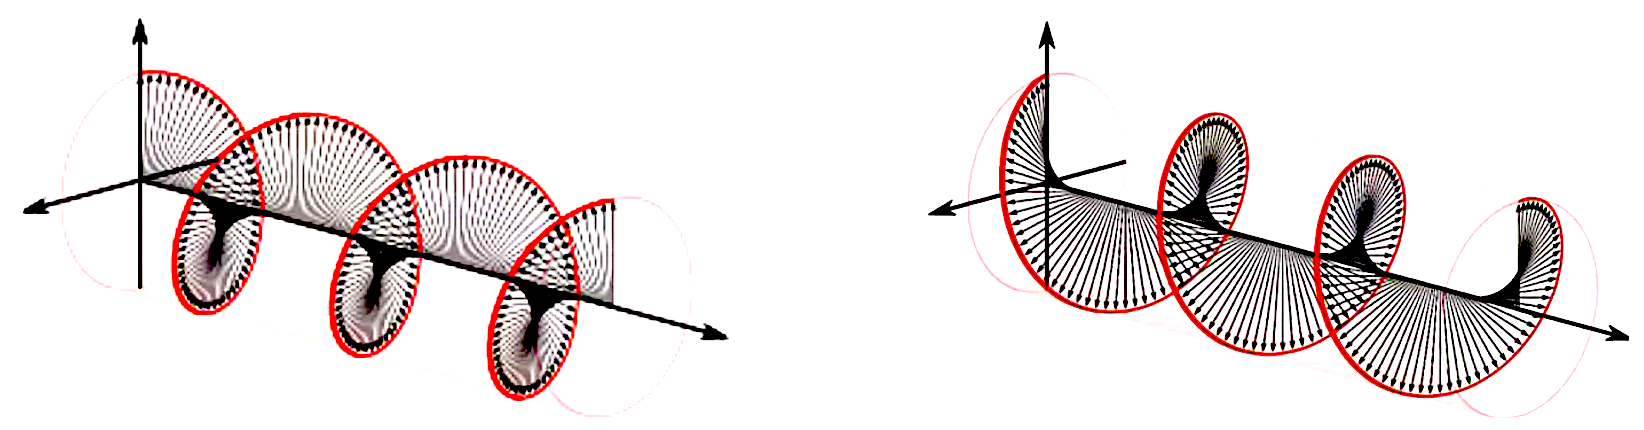
\includegraphics[width=0.3\textwidth]{/Users/vladbelousov/Desktop/Semestr_4-FP-NSU/ДфУ/Лекции_по_дням/image/9.png}
        \end{center}

        \[ \int_{ x_0 }^{x_1} f(x ) \eta(x ) dx = \int_{\tilde{x} - \delta_0}^{\tilde{x}- \delta_0} \underbrace{f(x)}_{>0} \underbrace{\eta( x)}_{>0} dx >0 - \text{противоречие}    \] 

        \[ \Rightarrow \forall x \in  [x_0, x_1] : f(x) = 0  \] 
    \end{proof}

    Из доказательства леммы следует, что доказана формула (2)
\end{proof}

\section{Случай понижения порядка в уравнении Эйлера}   

\[ \frac{\partial F}{\partial y} - \frac{d}{d x }  \frac{\partial F}{\partial y'} = 0 \quad  F=F(x,y(x),y'(x))  \] 

1) \(\displaystyle  F= f(x,y) \Rightarrow \frac{d}{dx }  \frac{\partial F }{\partial y'} (x,y') =0 \Rightarrow y= y(x)    \) 

2) \( \displaystyle F= F (x, y ') \Rightarrow \frac{\partial F }{\partial y} (x,y) =0 \Rightarrow \frac{\partial F }{\partial y'} (x,y') = C    \) 


3) \( F= F( y , y ') \) :

\[ \frac{\partial F }{\partial y } - \frac{d}{dx }  \frac{\partial F }{\partial y '} = 0 | \cdot y '     \] 

\[ y' \frac{\partial F }{\partial y } - \underbrace{y ' \frac{ \partial F }{\partial y '}}_{= \frac{d}{dx } \left( y ' \frac{\partial F }{\partial y '} \right)- y'' \frac{\partial F }{\partial y '} }    = 0 \] 

\[ y' \frac{\partial F }{\partial y } - \frac{d}{dx } \left( y ' \frac{\partial F }{\partial y '}  \right)+ y'' \frac{\partial F }{\partial y '}  = 0 \] 

Заметим, что: \( \displaystyle \frac{d}{dx }F(y,y')  = y' \frac{\partial F }{\partial y } + y '' \frac{\partial F }{\partial y '}   \) 

\[ \frac{d}{dx }  F - \frac{d}{dx } \left( y ' \frac{\partial F }{\partial y '}           \right) = 0 \Rightarrow \boxed{F- y ' \frac{\partial F }{\partial y '} = C}   \] 


\section{Решение задачи о брахистохроне}

\begin{center}
    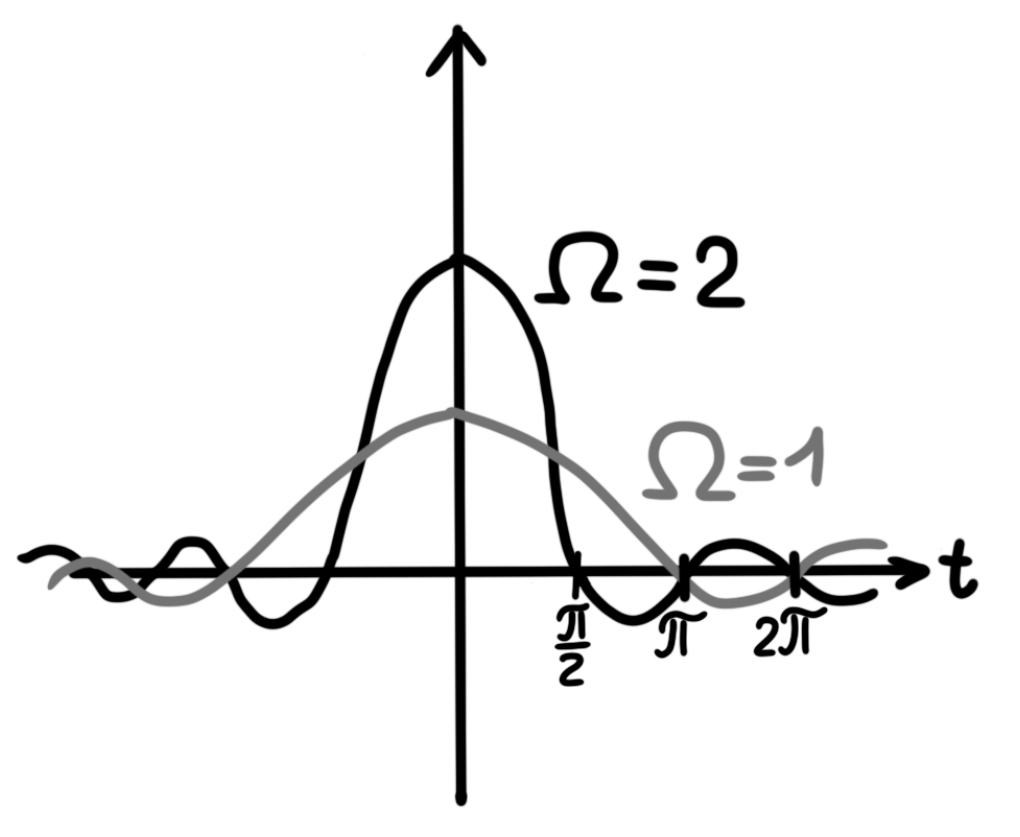
\includegraphics[width=0.3\textwidth]{/Users/vladbelousov/Desktop/Semestr_4-FP-NSU/ДфУ/Лекции_по_дням/image/10.png}
\end{center}

\[ \begin{cases}
\displaystyle I[y] = \int_{x_0}^{x_1} \frac{\sqrt{ 1+ (y ' (x)) ^2 )}}{\sqrt{2 g (y_0 - y (x))}} dx \\
y(x_0) = y_0, \text{ } y(x_1) = y_1
\end{cases} \] 

\[ \frac{\sqrt{1+ ( y ' ) ^2 } }{ \sqrt{2 g ( y_0 - y )} } - y ' \frac{1}{\sqrt{2 g ( y_0 - y )}} \frac{2 y '}{2 \sqrt{1 +( y ') ^2 } } = C    \] 

\[ \underbrace{\sqrt{1+ ( y ' ) ^2 } - (y ') ^2 \frac{1}{ \sqrt{1 + (y') ^2}}}_{\displaystyle \frac{1}{\sqrt{1+ (y ') ^2 }} } = C \sqrt{2g (y_0 - y )}  \] 

\[ 1= \underbrace{c ^2 2g}_{= \frac{1}{c_1}>0 } ( y_0 - y)( 1+ (y ') ^2) \] 

\[ c_1= (y_0 - y )(1 + ( y ' ) ^2 ) \Rightarrow \pm \sqrt{\frac{c_1}{y_0 - y }-1} = y ' \quad (3 )  \] 

\begin{center}
    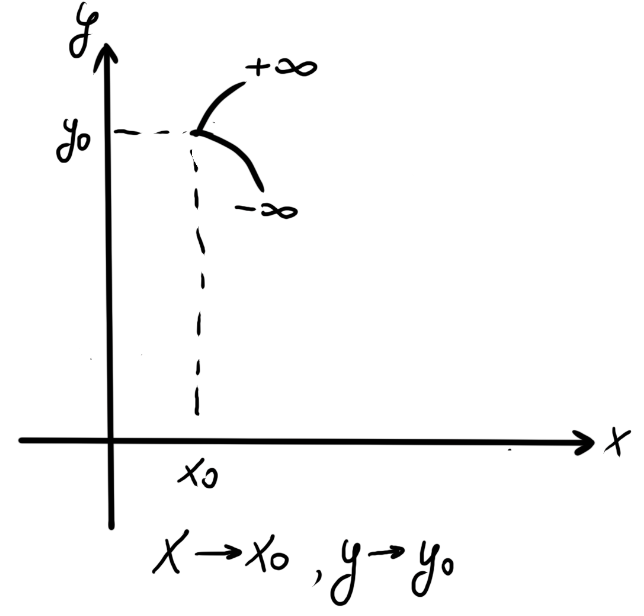
\includegraphics[width=0.3\textwidth]{/Users/vladbelousov/Desktop/Semestr_4-FP-NSU/ДфУ/Лекции_по_дням/image/11.png}
\end{center}

\[ 1+(y'(x)) ^2 = \frac{c_1}{y_0 - y(x)} \xrightarrow{x \to x_1} + \infty     \] 

\[ y ' ( x ) \xrightarrow{x \to  x_0} \underset{{\small \text{выбор}} : - }{\pm \infty}  \Rightarrow y ' (x )  \xrightarrow{x \to  x_0} - \infty      \] 

Если выбрать знак "+", то тело не сможет скатится в нужную точку 

\[ y ' = - \sqrt{\frac{c_1- y_0 + y }{y_0 - y } } \] 

Замена: \( \tilde{y }= y_0 - y (x) \):

\[ \tilde{y} '(x) = + \sqrt{\frac{c_1 - \tilde{y }}{\tilde{y }} }  \] 

Замена: \( \tilde{y } = c_1 z \): 

\[ c_1 z ' = \sqrt{\frac{c_1 - c_1 z }{c_1 z } }= \sqrt{\frac{1-z}{z } } \] 

Замена: \( z= \sin ^2 s, s \in  \left[ 0 , \frac{\pi}{2}  \right] \) 

\[ c_1 2 \sin s \cos s \cdot s' = \sqrt{ \frac{1- \sin ^2 s }{\sin ^2 s } }= \frac{\cos s }{\sin s } \text{ } (\text{знак определили из интервала s} )   \] 

\[ 2 c_1 \sin ^2 s \frac{ds}{dx } =1     \] 

\[ \frac{dx }{ds }  = c_1 ( 1 - \cos (2s) ) \Rightarrow \boxed{x(s) = c_1 \left( s - \frac{1}{2 }  \sin 2s  \right)+c_2}   \] 

\[ y(x )= y_0 - \tilde{y } (x ) = y_0 - c_1z= y_0 - c_1 \sin ^2 s = y_0 - \frac{c_1}{2} ( 1 - \cos  2s) \]  

\[ \boxed{y(s )= y_0 - \frac{c_1}{2 }  ( 1 - \cos (2s))}   \] 

Замена: \( t = 2s , \text{}  t \in  ( 0 , \pi) \) 

\[ \begin{aligned}
    \begin{cases}
        \displaystyle x(t) = \frac{c_1}{ 2 }  ( t - \sin t ) + c_2  \\ 
        \displaystyle y(t)= y_0 - \frac{c_1}{2 }  ( 1 - \cos t)
    \end{cases}
    \quad , \quad t \in ( 0 , \pi)
\end{aligned} \]

\[ \begin{pmatrix}
x(t )\\
y (t)
\end{pmatrix} = \begin{pmatrix}
\frac{c_1}{2 }  + c_2 \\
y - \frac{c_1}{2} 
\end{pmatrix}= \begin{pmatrix}
-\frac{c_1}{2 } \sin t\\
\frac{c_1}{2}  \cos t 
\end{pmatrix} \quad t \in  (0 , \pi)\] 

\begin{center}
    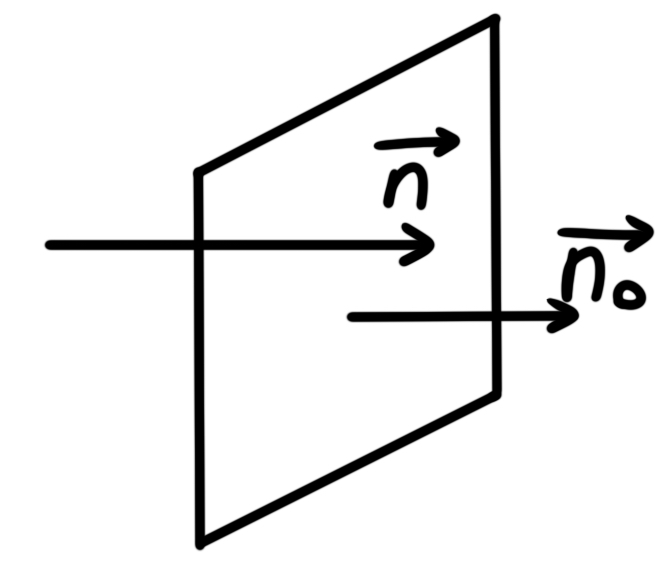
\includegraphics[width=0.5\textwidth]{/Users/vladbelousov/Desktop/Semestr_4-FP-NSU/ДфУ/Лекции_по_дням/image/12.png}
\end{center}

\[ \begin{aligned}
    t= 0 : 
    \begin{cases}
        x(0 ) = c_2 = x_0 \\
        y(0 ) = y_0
    \end{cases}
\end{aligned} \] 

\[ \begin{aligned}
    t= \pi: 
    \begin{cases}
        x(\pi ) = \frac{c_1}{2 }  \pi + c_2= \frac{c_1}{2 } \pi + x_0  \\
        y(\pi) = y_0 - c_1
    \end{cases}
\end{aligned} \] 

\begin{center}
    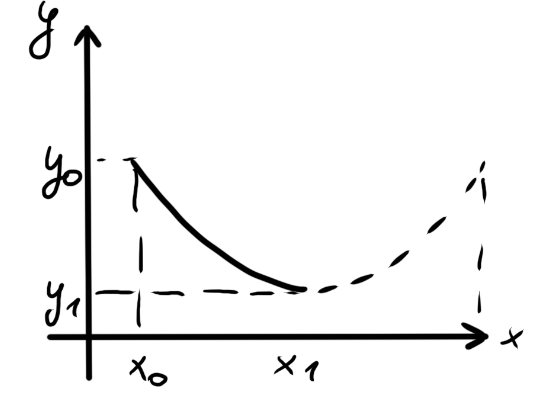
\includegraphics[width=0.3\textwidth]{/Users/vladbelousov/Desktop/Semestr_4-FP-NSU/ДфУ/Лекции_по_дням/image/13.png}
\end{center}

Теперь возьмем "+" ( формула (3)): 

\[ y ' = \sqrt{\frac{ c_1 - y_0 + y }{y_0 - y } }\quad (5 ) \] 

\[ \tilde{y } (x ) = y_0 - y (x ) \Rightarrow \tilde{y } ' = - \sqrt{\frac{ c- \tilde{ y } }{\tilde{y }}}   \]  

Делаем те же действия (замены) и получаем такие же \( x(s), y ( s ) \) с различием только в интервале для t: 

\[ \begin{aligned}
    \begin{cases}
        x(t)  = \frac{C_1}{ 2 }  ( t- \sin t ) + x_0 \\
        y(t ) = y_0 - \frac{c_1}{2 }  ( 1- \cos  t )            
    \end{cases}
    \quad ,\quad t \in ( 0 , 2 \pi ) \Rightarrow \text{ циклоида полная }  
\end{aligned} \]  

\begin{center}
    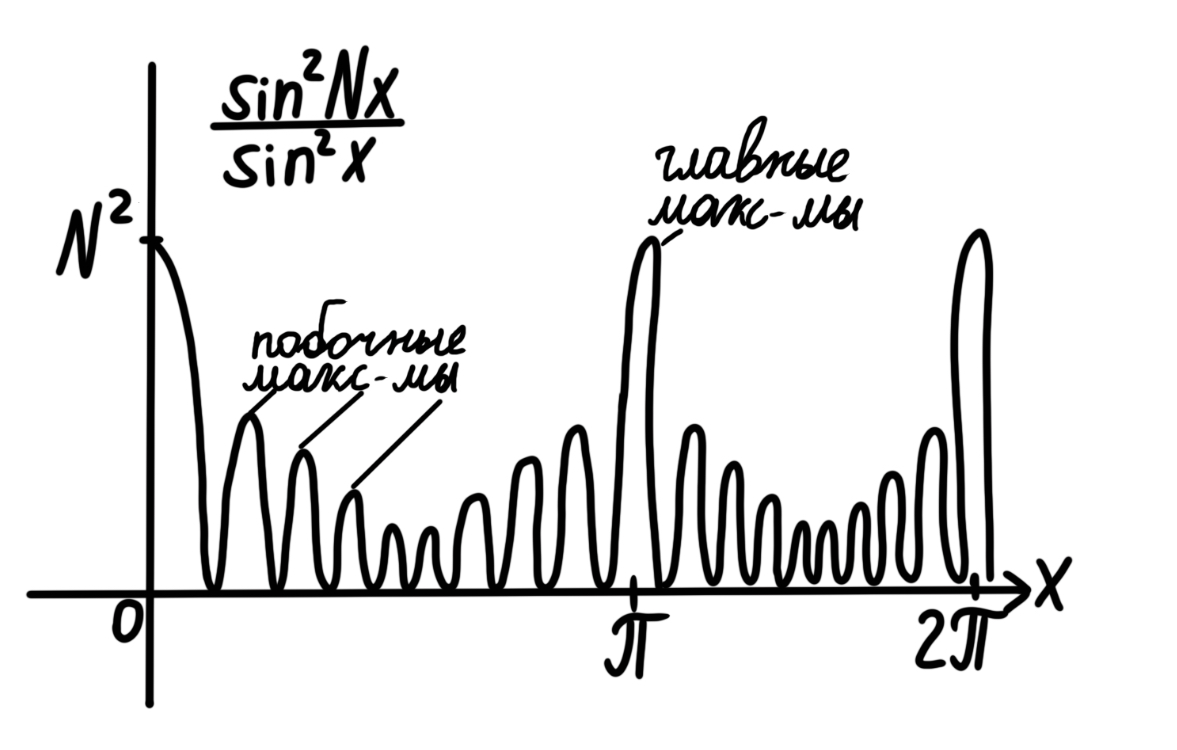
\includegraphics[width=0.5\textwidth]{/Users/vladbelousov/Desktop/Semestr_4-FP-NSU/ДфУ/Лекции_по_дням/image/14.png}
\end{center}

\newpage

\section{Решение задачи о поверхности вращения наименьшей площади}

\begin{center}
    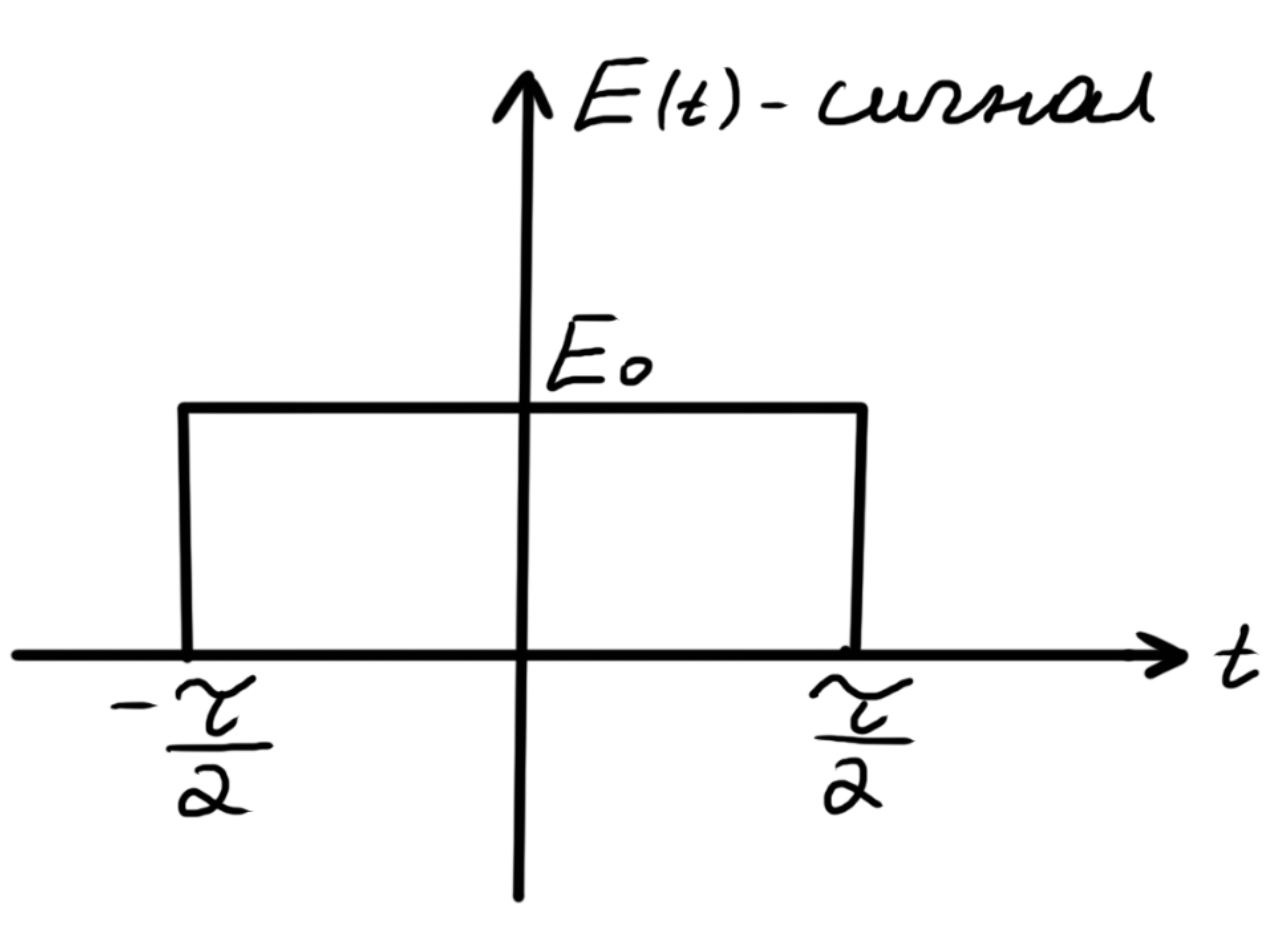
\includegraphics[width=0.3\textwidth]{/Users/vladbelousov/Desktop/Semestr_4-FP-NSU/ДфУ/Лекции_по_дням/image/15.png}
\end{center}

\[ \begin{cases}
I[ y ] = \int_{x_0}^{x_1} 2 \pi y(x )  \sqrt{1 + (y '(x ) ^2 )} \\ 
y( x_0 ) = y_0 , \text{ }  y ( x_1 ) = y_1 
\end{cases} \] 

\[ F- y \frac{\partial  F }{\partial   y' } = C   \] 

\[ 2 \pi y \sqrt{ 1 + (y' ) ^2 } - y ' 2 \pi y \frac{2 y '}{ 2 \sqrt{1 + ( y ') ^2 }} = C  \] 

\[ 2 \pi y \underbrace{\left( \sqrt{1 + (  y') ^2 } - \frac{ (y ' ) ^2 }{\sqrt{1 + ( y ' ) ^2 }}  \right)}_{= \frac{1}{\sqrt{ 1 + ( y ' ) ^2 }} } = C \] 

\[ ( 2 \pi y  ) ^2 = c ^2 ( 1 + ( y '   ) ^2 ) \] 

1) \( c= 0 \Rightarrow y(x )  =0  \) - решение, если \( y_0 = y_1 = 0 \) 

2) \( c \neq 0 \Rightarrow \left(  \frac{y}{c_1 }     \right) ^2 = 1 + ( y ' ) ^2 \Rightarrow y ' = \pm  \sqrt{\frac{ y ^2 }{c_1 ^2} - 1  }, \text{ }  c_1 = \frac{c}{2 \pi} > 0         \) 

\[ y( x ) = \mathrm{ch}  z(x  ) c_1 , \text{ }  z> 0 \]  

\[ c_1 \mathrm{sh } z \cdot z ' (x )   =\pm \underbrace{ \sqrt{\mathrm{ch} ^2 z - 1  }}_{= \mathrm{sh} z  }   \Rightarrow c_1 z'  = \pm 1   \] 

\[ z= \pm  \frac{ x+ c_2 }{c_1} \Rightarrow y ( x )  = c_1 \mathrm{ch} \left( \frac{x+c_2 }{c_1}  \right)  - \text{цепная линия}  \] 

\begin{center}
    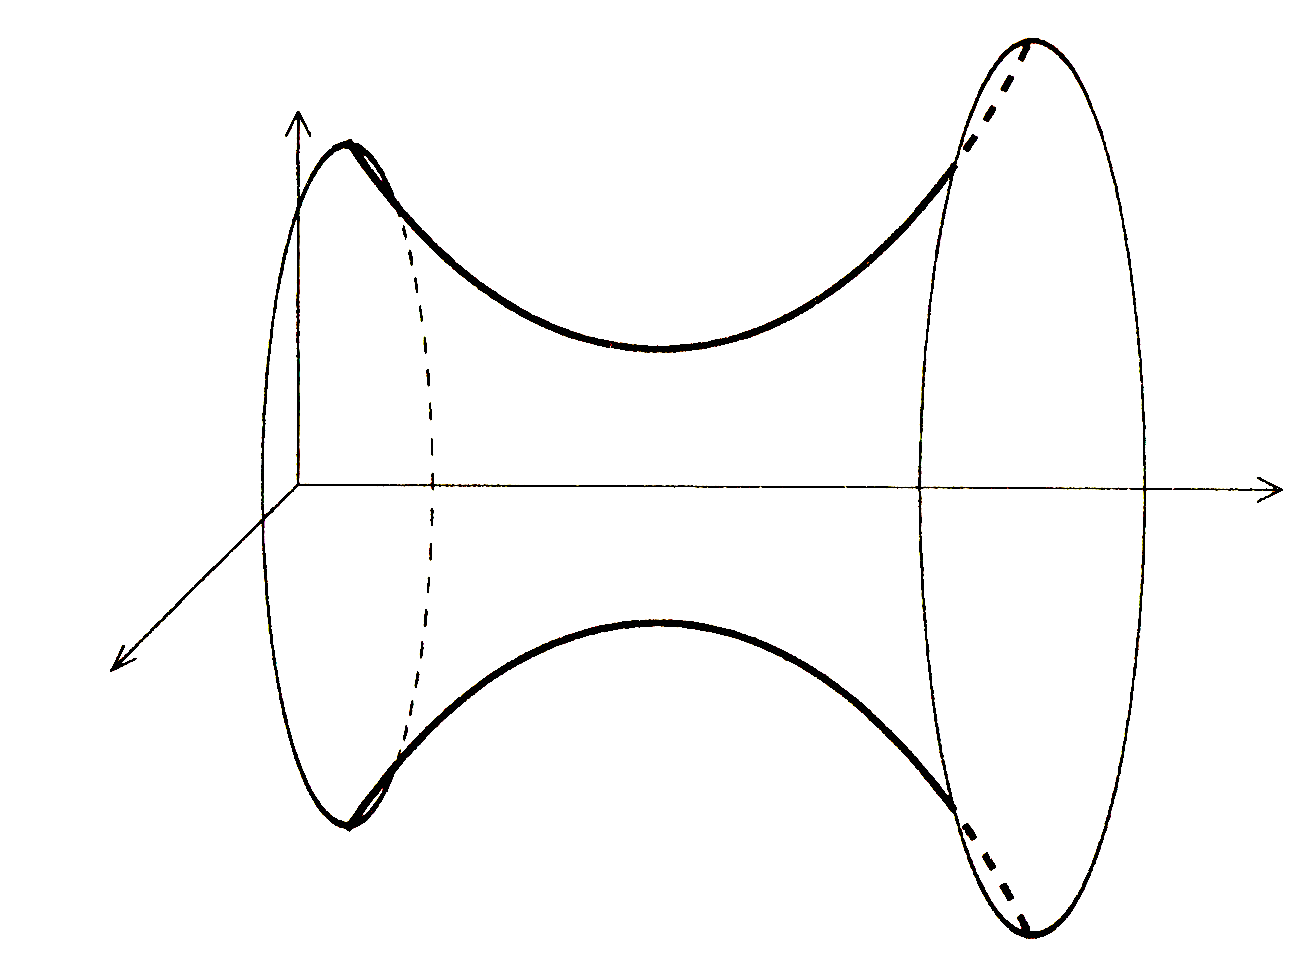
\includegraphics[width=0.4\textwidth]{/Users/vladbelousov/Desktop/Semestr_4-FP-NSU/ДфУ/Лекции_по_дням/image/16.png}
\end{center}



\section{Вариационная задача с несколькими функциями}

\[ I[y_1, \ldots, y_n ] = \int_{x_0 }^{x_1 } F(x,y_1(x),y_1 ' (x), \ldots , y_n ( x ) , y _n '( x))dx  \] 

\[ \begin{cases}
    y_1(x_0 ) = y_{01} , \ldots , y_n ( x_0 ) = y_{0n } \\
    y_1(x_1 ) = y_{11} , \ldots , y_n ( x_1) = y_{1n }
\end{cases} \] 

Необходимое условие локального экстремума: 

Пусть \( \tilde{y }_1 (x ) ,\ldots, \tilde{y }_n( x )  доставляет функционалу локальному экстремуму ему, то есть: \)

\[ I [\tilde{y }_1, \ldots , \tilde{y}_n  ] \le I[y_1, \ldots , y_n ] , \text{ }  \forall y_2, \ldots , y_n \] 

Можно взять \( y_1   \) - любое: \( y_2=\tilde{y}_2, \ldots ,   \) 

\[\Rightarrow \underbrace{ I[\tilde{y}_1, \ldots, \tilde{y   }_n ]}_{Y[\tilde{y } _1] } \le \underbrace{I[y_1, \ldots, \tilde{y  }_n ]}_{Y[y_1 ]} \Rightarrow \frac{\partial F }{\partial  y_1} - \frac{d}{dx }  \frac{\partial  F }{\partial  y_1 '}= 0     \]  

Аналогично: \( \frac{\partial F }{\partial  y_j }- \frac{d}{dx }  \frac{\partial F }{\partial  y ' _j} = 0   \) 


%%-------------------------------%%

% Закрытие документа, если файл компилируется отдельно
\ifdefined\mainfile
    % Если это основной файл, не нужно заканчивать документ
\else
    \end{document}
\fi